\chapter{Функционално програмиране}

\setcounter{section}{21}

\section {Уводни задачи}

\begin{enumerate}

  \item Да се дефинира функция, която намира лицето на триъгълник по дадени: а) дължини на страна и височина към нея; б) три страни.
  
  \item Да се дефинира функция, която по двойка $(x,y)$ коррдинати на точка от равнината намира на кой квадрант принадлежи точката. Да се разгледат случаите, когато точката принадлежи на някоя от координатните оси или съвпада с центъра на координатната система.

  \item Да се дефинира функция, която  има стойност истина, ако посоченото условие е вярно и стойност - лъжа, в противен случай:

	\renewcommand{\theenumii}{\Alph{enumii}}

	\begin{enumerate}[label=\alph*)]%[a)] % a), b), c), ...
			 \item цялото число p се дели на 4 или на 7;
			 \item уравнението $ax^2 + bx + c = 0 (a \neq 0)$ няма реални корени;
			 \item точка с координати (a, b) лежи във вътрешността на кръг с радиус 5 и център (0, 1); г) точка с координати (a, b) лежи извън кръга с център (c, d) и радиус f;
			 \item точка принадлежи на частта от кръга с център (0, 0) и радиус 5 в трети квадрант;
			 \item точка принадлежи на венеца с център (0, 0) и радиуси 5 и 10;
			 \item x принадлежи на отсечката [0, 1];
			 \item x е равно на max \{a, b, c\};
			 \item x е различно от max \{ a, b, c\};
			 \item нито едно от числата a, b и c не е положително;
			 \item цифрата 7 влиза в записа на положителното трицифрено число p;
			 \item цифрите на трицифреното число m са различни;
			 \item поне две от цифрите на трицифреното число m са равни помежду си;
			 \item цифрите на трицифреното естествено число x образуват строго растяща или строго намаляваща редица;
			 \item десетичните записи на трицифрените естествени числа x и y са симетрични;
			 \item естественото число x, за което се знае, че е по-малко от 23, е просто.
  \end{enumerate}

  \item Да се напише функция, която намира броя на цифрите в десетичния запис на дадено естествено число.
  
  \item Да се напише функция, която намира сумата на цифрите в десетичния запис на дадено естествено число.
  
  \item Да се дефинира функцията $pow(x,k)=x^k$ за цели положителни числа $x$ и $k$.
  
  \item Да се напише функция, която по дадени естествено число $x$ и едноцифрено числа $k$ намира а)дали $k$ се среща в десетичния запис на $x$ и б) колко пъти $k$ се среща в десетичния запис на $x$.
  
  \item Да се напише функция, която проверява дали дадена година е високосна. (вж. задача 2.12. в \cite{sbornik})
  
  \item Да се напише функция, която по дадено естествено число n ($n \geq 1$) намира броя на тези елементи от серията числа $i^3 + 13 \times i \times n + n^3$ , $i = 1, 2, ..., n$, които са кратни на 5 или на 9.

  \item Да се дефифира функция, която по естествени числа $n$ и $k$ намира дали $n$ е точна степен на числото $k$.

  \textit{Упътване: Разделете променливата $n$ на променливата $k$ ``колкото пъти е възможно'' и проверете дали $n$ достига единица или някое друго число след края на процеса. Използвайте оператора за намиране на остатък при целочислено деление и оператора за целочислено деление.}

  \item Едно положително цяло число е съвършено, ако е равно на сумата от своите делители (без самото число). Например, 6 е съвършено, защото 6 = 1+2+3; числото 1 не е съвършено. Да се дефинира функция, която проверява дали дадено положително цяло число е съвършено.


  \section {Конструиране на списъци}

  \item Да се съставят следните списъци:
	\renewcommand{\theenumii}{\Alph{enumii}}

	\begin{enumerate}[label=\alph*)]%[a)] % a), b), c), ...
			 \item Първите $n$ четни числа;
			 \item Първите $n$ члена на аритметична прогресия с първи член $a$ и разлика $d$;
			 \item $[1!, 2!, ..., n!]$ за дадено $n$;
			 \item Всички четни числа;
			 \item Всички членове на аритметична прогресия с първи член $a$ и разлика $d$;
			 \item $[1!, 2!, ...]$ (безкраен списък)
  \end{enumerate}

  \item Да се дефинира функция, която по дадено естествено число $n$ връща списък с цифрите му, четени отдясно на ляво.

  \item(*) Да се дефинира функция, която по дадено естествено число $n$ връща списък с цифрите му, четени отдясно на ляво, без повторения на елементите на списъка.

  \item Едно положително цяло число е съвършено, ако е равно на сумата от своите делители (без самото число). Например, 6 е съвършено, защото 6 = 1+2+3; числото 1 не е съвършено. Да се дефинира функция, която създава списък с  всички съвършени числа, ненадминаващи дадено положително цяло число в параметър $n$.
  
  \item Да се дефинира функция $histogram$, която по символен низ $s$ връща списък от двойки $(c_i,n_i)$, където $c_i$ са различните символи от $s$, а $n_i$ е броя на срещания на $c_i$ в $s$. Например, $histogram \: "abracadabra" \rightarrow [(a,5), (b,2), (r,2), (c,1), (d,1)]$. Използвайте помощни функции.
\end{enumerate}

\section {Работа със списъци и образци}

\begin{enumerate}[resume]

	\item Дефинирайте функция $say$, която по едноцифрено цяло число връща неговото наменование. Например, $say \: 3 \rightarrow "three"$.

	\item Да се дефинира функция, която по два списъка намира дължината на най-дългия им общ префикс.

	\item Да се дефинира функция $countEvenOdd \: l$, която за списъка от цели числа $l$ връща наредена двойка от броя на четните и броя на нечетните числа в $l$.

	\item Да се дефинира функция $pivot \: l \: x$, която за списъца от числа $l$ и числото x връща наредена двойка $(l_1,l_2)$, където $l_1$ е списък от елементите на $l$, по-малки от $x$, а $l_2$ е списък от елементите на $l$, по-големи или равни на $x$.
	
	\item Да се дефинира функция, която в даден низ замества всички малки латински букви със съответните им големи латински букви.
	
	\item Да се дефинира функция, която проверява дали даден низ е палиндром, т.е. дали се е еднакъв при четене от ляво на дясно и от дясно на ляво.
	
	\item Да се дефинира функция, която по даден списък от цели числа $l$ връща списък от всички двойки $(a,b)$ от $l$, за които $a$ и $b$ са съседни елементи в $l$ и $a < b$.
	
	\item Да се дефинира функция \code{groupsof l x}, която разделя списъка $l$ на групи от по $x$ елемента. 
	
	Например, $groupsof \: [1,2,3,4,5,6,7,8] \: 3 \rightarrow [[1,2,3],[4,5,6],[7,8]]$.

	\item Да се дефинира функция $flatten \: \: l :: [[a]] \rightarrow [a]$, която получава списък от списъци и връща списък, който съдържа всички елементи на входните списъци.

	\item Да се дефинира функция $decode \: l :: [(Int,a)] \rightarrow [a]$, която получава списък от двойки и връща списък, който съдържа всички елементи на входния списък, като всеки елемент се повтаря толкова пъти, колкото е указано в първия елемент на двойката.

	\item Да се дефинира функция $pack \: l :: [a] \rightarrow [[a]]$, която получава списък и връща списък от списъци, като всеки от тях съдържа всички последователни еднакви елементи на входния списък.
	
	Например, $pack \: [1,1,1,2,2,3,4,4,4,4] \rightarrow [[1,1,1],[2,2],[3],[4,4,4,4]]$.

	\item Да се дефинира функция $encode \: l :: [a] \rightarrow [(Int,a)]$, която получава списък и връща списък от двойки, където първият елемент на двойката е броят на последователните еднакви елементи от входния списък, а вторият елемент е самият елемент.
	
	Например, $encode \: [1,1,1,2,2,3,4,4,4,4] \rightarrow [(3,1),(2,2),(1,3),(4,4)]$.

	\item Да се дефинира функция \code{remove x l}, която премахва (а) първото срещане на елемента $x$ от списъка $l$ и (б) всички срещания на елемента $x$ от списъка $l$.
		
	\item Да се дефинира функция \code{removeDuplicates l}, която премахва всички повторения на елементите на списъка $l$.
	
	\item За даден списък $L$, да се намерят елементите на списъка, чиято стойност е по-голяма от сумата на предхождащите ги елементи. Пример $[1,2,5,9,16] \rightarrow [1,2,5,9]$.
	
	\item Да се дефинира функция \code{mergeevenodd l1 l2}, която получава два списъка от цели числа $l1$ и $l2$ и връща списък, чиито елементи на четни позиции са елементите на $l1$, а тези на нечетни позиции са елементите на $l2$. Пример: \code{mergeevenodd [1,2,3] [4,5,6] -> [1,4,2,5,3,6]}.


\end{enumerate}

\section {Функции от по-висок ред}

\begin{enumerate}[resume]
	\item Направете и тествайте собствена реализация на функциите \code{map}, \code{filter} и \code{fold(l,r,l1,r1)}.
	\item Нека е даден списък \code{l::[(Int,Int,Int)]} с тройки $(a_i,b_i,c_i)$. С помощта на \code{map}, \code{fold} и \code{filter} да се намерят:
	
	\begin{enumerate}[label=\alph*)]
		\item Списъка от сумите на елементите на тройките $[(a_i+b_i+c_i)]$
		\item Тройка от сумите на отделните компоненти на елемнтите на \code{l}, $(\sum a_i,\sum b_i, \sum c_i)$
		\item Броя на тройките, за които $a_i+b_i>c_i$
		\item Дали има поне една тройка, за която $a_i=b_i=c_i$ (\code{True} или \code{False})
	\end{enumerate}
	\item За списък от числа $L$ да се намери списък с само с тези числа, които съвпадат с поредния си номер в $L$. Например $[1,5,3,4,2] \rightarrow [1,3,4]$.

	\item За списък от числа $L$ да се намери списък със сумите на всички двойки последователни елементи на $L$. Например $[1,5,3,4,2] \rightarrow [6,8,7,6]$. \emph{Упътване: Използвайте \code{zip}.}
	
	\item С помощта на \code{zipWith} да се дефинира функция \code{sums :: [Int] -> [Int]}, която по списък от числа $L=l_1,l_2,l3,...$ намира списъка $S=l_1,(l_1+l2_),(l_1+l_2+l_3),...$. 
	
	\item Да се дефинира функция \code{separate :: (a->Bool) -> [a] -> ([a],[a])}, която по предикат $p$ и списък $l$ връща двойката \code{(pref,suf)}. \code{pref} е най-дългият възможен префикс, такъв че всички негови елементи увовлетворяват \code{p}. \code{suf} е останалата част от списъка $l$. Например, \code{separate even [2,4,6,7,8,10] -> ([2,4,6],[7,8,10])}. \emph{Забележка: вижте функцията \code{break}  в \code{Prelude}.}
	
	\item \label{zad:split}Да се дефинира функция \code{split :: (a->Bool) -> [a] -> [[a]]}, получваваща предикат \code{p} и списък \code{l}. Елементите на \code{l}, удовлетворяващи \code{p}, се считат за ``разделители'' в \code{l} и списъкът се разделя на части, обособени от тези разделители. Например:
\begin{lstlisting}[basicstyle=\small,language=Haskell]
split (==',') "part1,part 2,part3" 
             -> ["part1","part 2","part3"]
\end{lstlisting}
\end{enumerate}

\begin{mdframed}[hidealllines=true,backgroundcolor=gray!20]
На лекции разглеждаме модел на лабиринт, сържащ цел и препятсвия.
\begin{lstlisting}[basicstyle=\small,language=Haskell]
type Pos = (Int, Int)
  
data Tile = Road | Wall | Gold
            deriving (Show, Eq)  
data Game = Game { pos :: Pos, world :: [[Tile]]}
            deriving (Show)
myWorld :: Game = Game { pos = (0, 0), 
                         world = [[Road, Wall, Gold], 
                                  [Road, Wall, Road], 
                                  [Road, Road, Road]]}
\end{lstlisting}
\begin{center}
	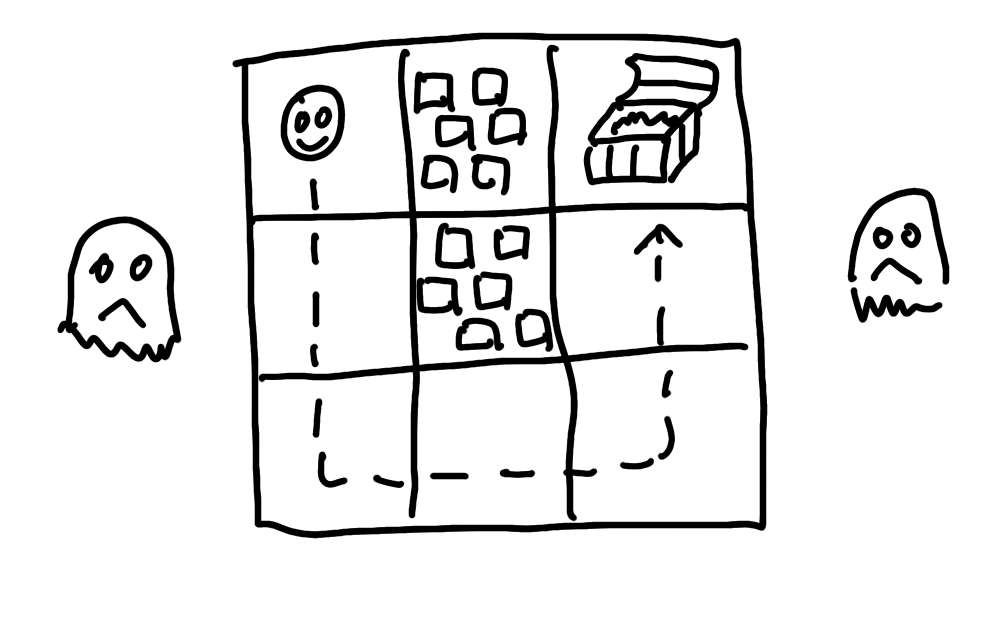
\includegraphics[width=4cm]{images/maze}	
\end{center}

Следите функции ``придвижват'' играча в лабиринта:

\begin{lstlisting}[basicstyle=\small,language=Haskell]
left (Game (x, y) w) = Game (x-1, y) w
right (Game (x, y) w) = Game (x+1, y) w
up (Game (x, y) w) = Game (x, y-1) w
down (Game (x, y) w) = Game (x, y+1) w	
\end{lstlisting}

И помощни функции при изследване на играта:

\begin{lstlisting}[basicstyle=\small,language=Haskell]
foundGold  :: Game -> Bool
foundGold  (Game (x,y) w) = (w !! y) !! x == Gold
stuck  :: Game -> Bool
stuck  (Game (x,y) w) = dead w (x, y)
dead :: [[Tile]] -> Pos -> Bool
dead w (x, y) = x < 0 || x >= length w ||
                y < 0 || y >= length w || 
                (w !! y) !! x == Wall
move :: Game -> (Pos -> Pos) -> Maybe Game
move (Game p w) mv = if dead w (mv p) 
                       then Nothing 
                       else Just $ Game (mv p) w
\end{lstlisting}

\end{mdframed}

\begin{enumerate}[resume]
	\item С помощта на \code{map}, \code{mapMaybe}, \code{filter} и \code{fold} да се намерят:
	\begin{enumerate}[label=\alph*)]
		\item Броя на препятсвията в даден лабиринт
		\item Броя съседи на целта, които не са препятсвия
		\item Дали целта е оградена изцяло от препятствия (\code{True} или \code{False})
	\end{enumerate}

	\item(*) С помощта на \code{foldr} да се дефинира функция, която проверява дали дали даден списък от числа \code{l::[Int]} е нареден във възходящ ред. \emph{Упътване: Използвайте двойка \code{(Bool,Int)} за акумулатор.}

\end{enumerate}

\section {$\lambda$ функции}

\begin{enumerate}[resume]
	\item Да се дефинира функция \code{caseof :: [a->Bool] -> [a->b] -> a->b}. Функцията приема $k$ на брой предиката над $a$ и $k$ на брой функции $a\rightarrow b$. Функцията \code{caseof} връща функция, която приема елемент $x$ от тип $a$ и връща резултата от първата функция, за която предикатът е изпълнен за $x$. Ако няма такава функция, функцията връща резултата от последната функция в списъка. Например, функцията:
\begin{lstlisting}[basicstyle=\small,language=Haskell]
myf = caseof [even, odd] [(\x -> x+1), (\x -> x-1)]
\end{lstlisting}
	ще увеличава с единица четните числа и ще намалява с единица нечетните числа.
		
	\item   Да се дефинира функция \code{createfn :: [(a,b)]->a->b}, която по даден списък от двойки $(a_i,b_i)$, връща функция $f:a \rightarrow b$ дефинирана за всички $a_i$, така че $f(a_i)=b_i$. Например:

\begin{lstlisting}[basicstyle=\small,language=Haskell]
createfn [(1,2),(2,4),(3,6)] 2 -> 4
\end{lstlisting}

\item Да се дефинира функция \code{integrate :: (Double->Double) -> Int -> Double -> Double -> Double}, която по функция $f: Double \rightarrow Double$ и цяло положително число $N$ връща $i(a,b)$ от тип $i:Double \times Double \rightarrow Double$, изчисляваща приближено стойността на определния интеграл $\int_{a}^{b} f(x) dx$ (приемайки, че такъв съществува) по метода на трапеците, по-специално Chained trapezoidal rule\cite{trapezoidal} с $N$ на брой подинтервала. (вж. фиг. \ref{fig:trapezoidal})

\section {Вход/Изход}


\begin{mdframed}[hidealllines=true,backgroundcolor=gray!20]
\textbf{Пренасочване на стандартния вход и изход}

Когато една програма се изпълнява от операционната система, тя получава достъп за четене до поток от данни, неречен ``стандартен вход'' и достъп за писане до ``стандартен изход''. Ако програмата е стартирана в терминална сесия под Posix операционни системи (Mac OS, Linux) или Windows, стадртният вход се състои от поредицата символи, въведени от потребителя чрез клавиатурата. Стандртният изход се визуализира под формата на символи на терминалния прозорец. Това позволява така наречените ``конзолни проложения'', които са предвидени да работят в терминал, да реализират диалогов интерфейс с потребителя. На езика C++, стандартния вход и изход са достъпни чрез потоците \code{cin} и \code{cout}, дефинирани в \code{iostream}. На езика Haskell, достъп до стандартният вход и изход се осъществява чрез функции като \code{getLine}, \code{putStr} и \code{putStrLn}.

Операционните системи позволяват стандартния вход да бъде пренасочен така, че вместо от въведените чрез клавиатурата символи, входът да се състои от съдържанието на файл или от изхода на друга програма. Стандартният изход може да бъде пренасочен така, че вместо да се визуализира на терминала, да се запише във файл или да бъде предаден като вход на друга програма.

При Posix операционните системи, пренасочването на входа от файл или изхода към файл става така: 
\begin{lstlisting}[basicstyle=\small,language=bash]
./myprog < input.txt
./myprog > output.txt
\end{lstlisting}

Съответно, пренасочването на изхода на една програма като вход на друга става така:
\begin{lstlisting}[basicstyle=\small,language=bash]
ls -l | ./myprog
\end{lstlisting}
При тази команда, изходът на командата \code{ls} се подава като вход на програмата \code{myprog}.

Под Windows, пренасочването на входа и изхода от файл става по аналогичен начин:
\begin{lstlisting}[basicstyle=\small,language=bash]
myprog.exe < input.txt
myprog.exe > output.txt
\end{lstlisting}
\end{mdframed}

\item Да се деифнира програма, която прочита изхода на командата \code{ls -l} под MacOS и Linux или \code{dir} под Window и извежда на стадартния изход:
\begin{enumerate}[label=\alph*)]
	\item Броят на файловете и броят на поддиректориите в текущата директория
	\item Броят на файловете в текущата директория с разширение \code{.hs}
	\item Името на най-големия файл в текущата директория
	\item Името на най-новия файл в текущата директория
\end{enumerate}

\begin{mdframed}[hidealllines=true,backgroundcolor=gray!20]
\textbf{Форматът CSV}


Форматът ``Comma Separated Values (CSV)'' е текстов формат за представяне на таблични данни. В CSV формат, всеки ред от таблицата се представя като поредица от стойности, разделени със запетаи. 

Например:
\begin{verbatim}
Kalin Georgiev,M,01-01-1981
Maria Ivanova,F,05-05-2003
\end{verbatim}

Ако в рамките на дадена стойност се съдържа символът за запетая, за да не се интерпретира той като разделител, цялата стойност се поставя в двойни кавички. От друга страна, ако искаме самият низ да съдържа двойни кавички, то всяка дойна кавичка в него ограждаме с други две. Например следния низ:
\begin{verbatim}
"Hello """world""", have a nice day!"
\end{verbatim}
се интерпретира като стойността \verb#Hello "world", have a nice day!#.

\end{mdframed}

\item Да се дефинира функция \code{parseCSV :: String -> [[String]]}, която по даден ред от \code{csv} файл, представен като символен низ, връща списък от символни низове, представляващи стойностите му, като се разглеждат случаите на стойности, оградени с двойни кавички.

Разгледаната в задача \ref{zad:split} функция \code{split} разеделя символния низ спрямо даден разделител, в случая запетая. Резултатът от функцията може да се обработи допълнително:
\begin{enumerate}[label=\alph*)]
	\item Да се слее в един низ всяка редица от съседни елементи $a_i,a_{i+1},...,a_k$, такава че (1)$a_i$ започва с двойна кавичка;  (2)$a_k$ завършва с двойна кавичка; (3)никой от останалите $a_{i+1},...,a_{k-1}$ не започва или завършва с двойна кавичка. \emph{Упражнете се да ивършите тази трансформация чрез }\code{fold}.
	\item се заместят всички срещания на три последователни двойни кавички \verb#"""# с една двойна кавичка \verb#"#.
	\item Функцията да се преработи до \code{Maybe [[String]]} и да разглежда случаи на грешна употреба на кавички -- например две последователни кавички. Кои са всички възможни случаи на грешна употреба на кавички?
\end{enumerate}

\end{enumerate}


\section {Индуктивни типове данни}


\begin{mdframed}[hidealllines=true,backgroundcolor=gray!20]
\textbf{Gantt диаграми}

В управлнието на проекти, \href{https://en.wikipedia.org/wiki/Gantt_chart}{Gantt диаграмите} предоставят начин за визуализане на задачите, от които се състои даден проект, както и за анализ на зависимостите между тях. В тези диаграми всяка задача се характеризира с начало и продължителност. Някои от елемените на диграмата са ``обобщени задачи'', т.е. задачи, коието се сътоят от други задачи, както прости, така и обобщени.
\end{mdframed}

\begin{mdframed}[hidealllines=true,backgroundcolor=gray!20]
\textbf{Работа с дати в Haskell}

Модулът \href{https://hackage.haskell.org/package/time-1.14/docs/Data-Time-Calendar.html}{Data.Time.Calendar} дава удобни стредства за работа с дати от грегорианския календар. Основният тип \code{Day} представя конкретна дата от календара. Функции като \code{addDays} и \code{diffDays}, както и операторите за сравнение, дават възможност за изчисления с дати и сравнения на дати. Чрез \code{read} може да се иницилизира дата от символен низ във формат "YYYY-MM-DD". Функцията \code{show} позволява преобразуване на дата към символен низ.


Например, ако \code{start} е дадена дата в миналото, a \code{today} е текущата дата, то изразът \code{(addDays n start) > today} е истина, ако задача, която е започнала на дата \code{start} и е с продължителност n дни, е приключила към днешна дата.

\end{mdframed}

\begin{enumerate}[resume]
	\item Да се дефинира индуктивен тип \code{Task}, който представя задача от Gantt диаграма. Задачата може да бъде или проста (\code{SimpleTask}), или обобщена (\code{ComplexTask}). Простите задачи се характеризират с име, начало и продължителност. Обобщените задачи се характеризират с име и списък от подзадачи, които могат да бъдат както прости, така и обобщени. 
	
	Да се дефинира функция \code{completed :: Task -> Day -> Bool}, която по задача и дата връща дали задачата е приключила към тази дата. 

	\item Да се дефинира функция \code{duration :: Task -> Int}, която по задача връща нейната продължителност в дни. Продължителността на обобщена задача представлява разликата между дата на започване на най-рано започващата ѝ подзадачи и дата на приключване на най-късно приключващата ѝ подзадача. 
	
	\item \label{zad:tasksxml} Да се реализира извеждане на информацията за задача във \code{xml}-подобен формат. Например:
\begin{lstlisting}[basicstyle=\tiny,language=xml]
<complex descr="Take a course">
	<complex descr="Study">
		<simple descr="Read Textbook" start="2025-02-01" duration="20"/>
		<simple descr="Do homeworks" start="2025-02-10" duration="20"/>
	</complex>
	<simple descr="Take Exam" start="2025-03-01" duration="1"/>
</complex>
\end{lstlisting}

	\item(*)При извеждането на информацията за задача във \code{xml}-подобен формат, да се извърши индентация на вложените елементи, както е в примера на задача \ref{zad:tasksxml}.
	

\end{enumerate}


\section{Оценка на (аритметичен) израз}


\begin{mdframed}[hidealllines=true,backgroundcolor=gray!20]
\textbf{Оценка на изрази}


По време на лекции разработваме лексически анализатор, рекурсивен парсер и интепретатор на прост език, състоящ се от аритметични изрази от следния вид:
\begin{flushleft}
  \relscale{0.7}
  \begin{lstlisting}[mathescape]
  <expression> ::= <number> | (<expression> <operator> <exprerssion>)
  <number> ::= {0,..,9}+
  <operator> ::= + | - | * | /
  \end{lstlisting}
\end{flushleft}

За двата вида възможни изрази -- числова константа и приложение на двуместен аритметичен оператор, оградено в скоби -- дефинираме съответно възли в синтактично дърво. Дърво на израза построяваме от символен низ и оценяваме рекурсивно.

\end{mdframed}


\begin{enumerate}[resume]
	\item Интерпретаторът на изрази от лекции да се разшири с възможност за групиране на изрази в ``блокове'', започващи с ключовата дума \code{begin} и завършващи с ключовата дума \code{end}:
	\begin{flushleft}
	  \relscale{0.7}
	  \begin{lstlisting}[mathescape]
	<expression> ::= ... | begin (<expression>;)+ end
	  \end{lstlisting}
	\end{flushleft}
	
	Оценката на блок от изрази да се състои в последоватлено оценяване на всички изрази в блока и използване на онцеката на последния израз от блока като оценка на целия блок. Например: \code{begin 1; 2; 3; end} има оценка $3$.
	
\item Езикът, разработен на лекции, да се разшири с условен оператор от вида:
\begin{flushleft}
  \relscale{0.6}
  \begin{lstlisting}[mathescape]
<expression> ::= ... | if <expression> than <expression> else <expression>
  \end{lstlisting}
\end{flushleft}

Оценката на изразите от този вид е оценката на \code{expthen} или \code{exprelse} в зависимост от оценката на \code{condition}.



\item Интерпретаторът, разработен на лекции, да се разшири с възможност за присвояване на стойност на променлива:

\begin{flushleft}
\relscale{0.7}
\begin{lstlisting}[mathescape]
<expression> ::= ... | <assignment>
<assignment> ::= set <variable> = <expression>
\end{lstlisting}
\end{flushleft}

Примерни изрази на този език и съответния резултат от оценката им са:

\begin{lstlisting}[mathescape]
begin
  set x = (3*(1+2));
  x;
end
\end{lstlisting}
\emph{Оценка:} 9

\begin{lstlisting}[mathescape]
begin
  set x = 10;
  set y = 5*5;
  ((x*y)*2);
end
\end{lstlisting}
\emph{Оценка:} 500


\item(*) Интерпретаторът на аритметични изрази от лекции да се разшири с възможност за извеждане на стойност на израз на стандартния изход:
\begin{flushleft}
  \relscale{0.7}
  \begin{lstlisting}[mathescape]
<expression> ::= ... | print <exprression>
  \end{lstlisting}
\end{flushleft}

Оценката на израз от типа \code{print e} се намира като оценката на израза \code{e}, като освен това се произвежда извеждане на страндартния изход като страничен ефект. Всяка отделна стайност да бъде изведена на нов ред.

Примрер: Оценката на израза \code{print 1} ще е $1$ и ще доведе до извежане на ``1'' на стандарния изход. Оценката на 

\begin{flushleft}
  \relscale{0.7}
  \begin{lstlisting}[mathescape]
begin 
   print 1; 
   print 2; 
   print begin 3; 4; end;
end
  \end{lstlisting}
\end{flushleft}
ще доведе до извеждане на следните редове на стандартния изход: 
\begin{flushleft}
  \relscale{0.7}
  \begin{lstlisting}[mathescape]
1
2
4
  \end{lstlisting}
\end{flushleft}


\end{enumerate}
